% Appendix1 file from standard thesis template
\appendixtitle
\appendix
\chapter{SUPPLEMENTARY MATERIALS OF CHAPTER 2}

%This is now the same as any other chapter except that
%all sectioning levels below the chapter level must begin
%with the *-form of a sectioning command.
%
%\section*{More stuff}

The material in this document supplement the information presented in Chapter \ref{ch:largepsmalln}. Section \ref{sec:sol} presents the solutions to the lineups used in the chapter.  The choice of dimensions used in the Amazon Turk experiment is described in section \ref{sec:theory} .

%\section*{Supplemental material}

\section{Solutions to the Lineups} \label{sec:sol}
\begin{itemize}
\item The solution to the lineup at Figure \ref{lineup} is Plot 16. 
\item The solution to the lineup at Figure \ref{toth_lineup} is Plot 8.
\item The solution to the lineup at Figure \ref{fig:test_category_1d} is Plot 17.
\item The solution to the lineup at Figure \ref{fig:test_category} is Plot 20.

\end{itemize}

\section{Choice of dimensions} \label{sec:theory}

The experiment is set up with the 3 factors separation, dimension and projection dimension. To decide on the levels of dimension to use, we considered the distribution of the absolute difference of the sample group means, for data with two groups, no separation and projection dimension $d=1$. The same levels are used for data with 3 groups, $d=2$, and for data with separation. 

Let ${\blX}_{ij}$ denote the $j$-th observation in the $i$-th group where $j = 1, \dots, n; i=1, ..., g$. The ${\blX}_{ij}$'s are random noise, generated by drawing samples from a standard normal distribution. For this experiment, $g = 2$  and $n = 15$. The difference between the group means is given by $\overline{\mbox{X}}_{1.} - \overline{\mbox{X}}_{2.}$% and $$\overline{\mbox{X}}_{1.} - \overline{\mbox{X}}_{2.} \sim \hbox{Normal}(0, 1/n_1 + 1/n_2)$$ i.e. 
and $$\overline{\mbox{X}}_{1.} - \overline{\mbox{X}}_{2.} \sim \hbox{Normal}(0, 2/15)$$ Let 
$\mbox{U} = |\overline{\mbox{X}} _{1.} - \overline{\mbox{X}}_{2.}|$ 
where $\mbox{U} \sim \hbox{Half Normal}$ with scale parameter $ \sigma = \sqrt{2/15}$.
The expectation and the variance of $\mbox{U}$ are 
$E(\mbox{U} ) = \sigma \sqrt{2/\pi}$ and 
$Var(\mbox{U}) = \sigma^2 (1 - 2/\pi)$, respectively.

For $p$ dimensions, consider $p$ independent samples from the same distribution,  denoted as $${\blU}_m = |\overline{{\blX}}_{m1.} - \overline{{\blX}}_{m2.}|, ~~~ m=1, ..., p$$ where ${\blX} _{mij}$ is the $j$-th observation in the $i$-th group for the $m$-th dimension. The difference between the two group means projected into one dimension, is the sum over $p$ dimensions of the absolute difference between the means: $$\mbox{U}  = \sum_{m=1}^p {\blU}_m = \sum_{m=1}^p |\overline{{\blX}}_{m1.} - \overline{{\blX}}_{m2.}| $$ and by independence it follows that

$$\hbox{E}(\mbox{U}) = p \sigma \sqrt{2/\pi}, ~~~ 
\hbox{Var}(\mbox{U}) = p \sigma^2 (1 - 2/\pi)$$

\noindent Thus we expect to find this amount of separation between the projected sample means, for data sampled from populations with the same means.

Now consider data where there is some separation (equal to $2c)$ between the population means:

$${\blZ}_{1j} \sim \hbox{Normal}(-c, 1) $$
$${\blZ}_{2j} \sim \hbox{Normal}(c, 1) $$ 
giving $\overline{\mbox{Z}}_{1.} - \overline{\mbox{Z}}_{2.} \sim \hbox{Normal}(2c, 2/15)$. Then define $\mbox{Z}  = |\overline{\mbox{Z}}_{1.} - \overline{\mbox{Z}}_{2.}|$ where ${\mbox{Z}} \sim \hbox{Folded Normal Distribution}$ with scale parameter $ \sigma = \sqrt{2/15}$.  The expectation and the variance of $\mbox{Z}$ can be calculated to be:

$$\hbox{E}(\mbox{Z}) = \sigma \sqrt{2/\pi} \exp(- 2c^2/\sigma^2) + 2c[1 - \Phi(-2c/\sigma)]$$
$$\hbox{Var}(\mbox{Z}) = 4c^2 + \sigma^2 - (E(\mbox{Z}))^2$$

Suppose that only one of the $p$ dimensions is simulated from this distribution, and all of the rest are simulated from populations having identical means. Define $\mbox{V}$ as the sum of the absolute differences of the mean with one dimension of real separation as $$\mbox{V} = \sum_{m=1}^{p-1} \blU_m + {\blZ}$$ Then, by independence, it follows that:

$$\hbox{E}(\mbox{V}) = (p - 1) \sigma \sqrt{2/\pi} + \sigma \sqrt{2/\pi} \exp(- 2c^2/\sigma^2) + 2c[1 - \Phi(-2c/\sigma)]$$
$$\hbox{Var}(\mbox{V}) = (p - 1)\sigma^2 (1 - 2/\pi) + 4c^2 + \sigma^2 - \left( \sigma \sqrt{2/\pi} \exp(- 2c^2/\sigma^2) + 2c[1 - \Phi(-2c/\sigma)]\right)^2$$

In this experiment, $c = 3$ and $\sigma^2 = 2/15$. Therefore,
$$\exp(- 2c^2/\sigma^2) \approx 0 \qquad \hbox{and} \qquad \Phi(-2c/\sigma) \approx 0$$
Hence,
$$\hbox{E}(\mbox{V}) = (p - 1) \sigma \sqrt{2/\pi} + 6$$
$$\hbox{Var}(\mbox{V}) = (p - 1)\sigma^2 (1 - 2/\pi) + \sigma^2$$
As dimension $p$ increases for a fixed $n$, the spread of both U and V increases by a factor of $p$. The means of U and V also increase with a factor of $p$ but the expected value of the difference between U and V stays constant and is independent of dimension ($p$). 
%\begin{equation}
$$\hbox{E} (\mbox{V} - \mbox{U}) = (p - 1) \sigma \sqrt{2/\pi} + 6 - p \sigma \sqrt{2/\pi} = 6 - \sigma \sqrt{2/\pi}$$
%\end{equation}

Two $p$-dimensional datasets are generated with 30 observations in each dimension. The datasets are then divided into two groups with 15 observations in each group. For one set, data is obtained from random noise and hence there is no real separation between the two groups. But for the other set, one dimension among these $p$ is adjusted so that the data have some real separation between the groups in that dimension. The absolute difference of the means for each group in each of these $p$ dimensions is considered for both datasets. The absolute difference is considered as we are concerned with projections. These absolute differences between the groups are then summed over all the dimensions to obtain the absolute difference of means for the data. This process is repeated 1000 times. These 1000 sum of absolute differences are then plotted for the different values of $p$.

\begin{figure}[hbtp]
%\begin{figurehere}
   \centering
       \scalebox{0.70}{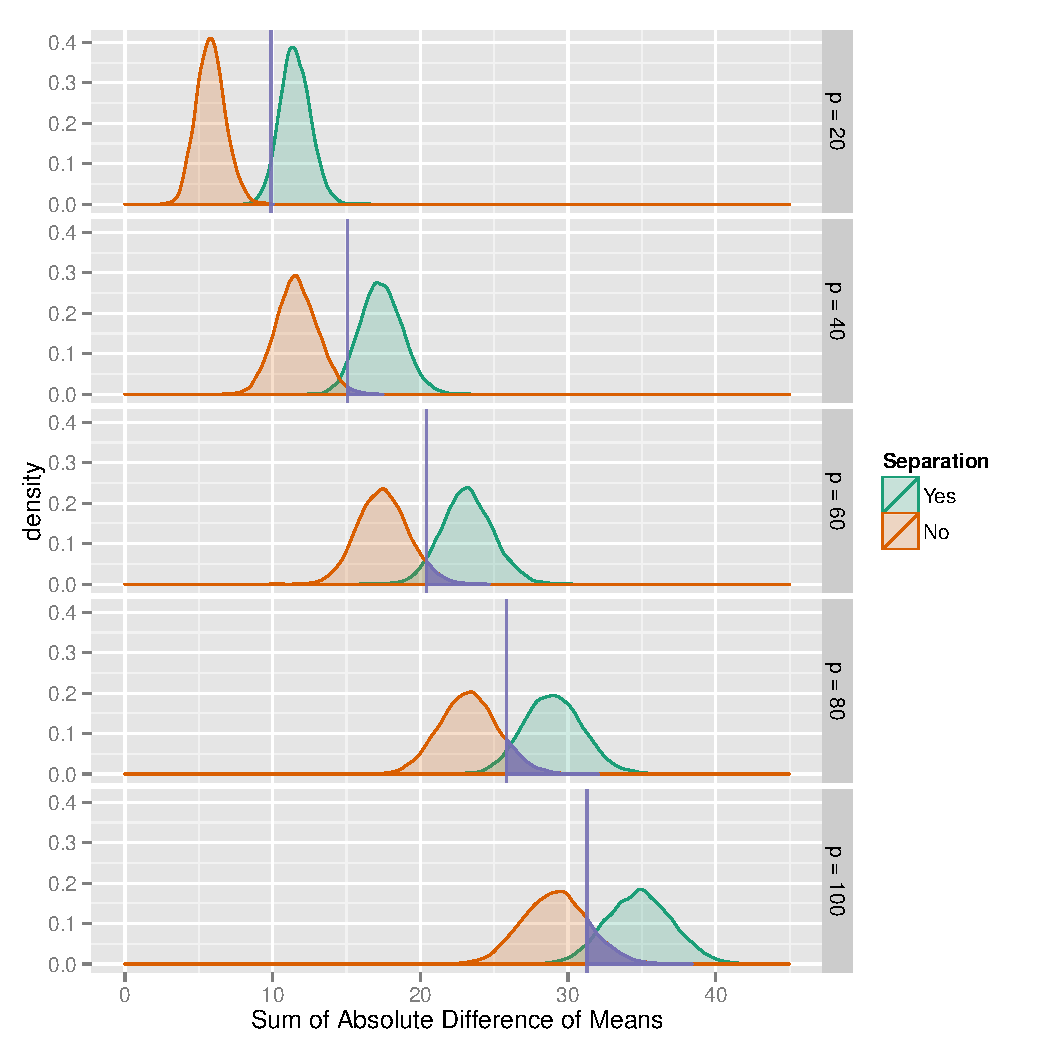
\includegraphics{sum-noise-real-2-rev.pdf}}
       \caption{Plot showing the distribution of the sum of absolute difference of means for data with and without separation for different dimensions. The distributions of data with real separation (V) and purely noise data (U) are shown in brown and green respectively with the dark purple line showing the 5th percentile of V. The dark purple area shows the area of U which is greater than the 5th percentile of V. The dark purple region ($\delta$) increases as dimension ($p$) increases. }
     \label{fig:dimen}
%\end{figurehere}
\end{figure}
 
Figure \ref{fig:dimen} shows the distribution of sum of absolute difference of means for data with and without separation for different dimensions. The distributions of data with and without separation are shown in brown and green respectively. The area of the distribution of pure noise which is above the 5th percentile of the distribution of data with separation is shown in dark purple.  Hence a 5\% error is allowed and let the area of the distribution of U greater than the 5th percentile of V be denoted by $\delta$. Mathematically, 

$$\hbox{P}[\mbox{U} > \mbox{V}_{\alpha}] = \delta$$ where $\mbox{V}_{\alpha}$ is the $100\alpha$-th percentile of V, where $\alpha = 0.05$.  It can be seen that the dark purple region increases with dimension ($p$). This indicates that as dimension increases, the distributions of data with or without separation gets closer. Hence it gets harder to detect real differences with higher dimensions. Fixing the area of the dark purple region ($\delta$) and calculating the dimensions to obtain the required region provides the choice of levels of dimension used in the experiment.

%Figure \ref{fig:dimen} illustrates this phenomenon. The distributions of data with separation (V) and without separation (U) are shown in red and blue respectively. As dimension ($p$) increases, the spread of both the distributions increases while the means are equally apart. As a result, the common region between the distributions increases, indicating the chance of obtaining a random separation for purely noise data increases with dimension($p$).

The various values of $\delta$ are chosen such that the distributions has no separation ($\delta \approx 0$) or has 1\%, 5\%, 10\% and 20\% common region. For each value of $\delta$, the procedure is repeated 100 times and Table \ref{tab:dimen} shows the summaries of the dimension ($p$) for each value of $\delta$.

\begin{table}[htbp]
\begin{center}
\caption{Numerical summaries of dimension $p$ for each value of $\delta$. As the common region $\delta$ increases, the median dimension required to obtain the region increases.}
\begin{tabular}{rrrr}
  \hline
  \hline
  $\delta$ & Median & 5th percentile & 95th percentile \\
  \hline
  0.0000001 & 24 & 19 & 28 \\
      0.01 & 41 & 38 & 44\\
   0.02 & 61 & 56 & 64 \\
     0.1 & 77 & 72 & 81\\   
     0.2 & 106 & 99 & 112\\ 
      \hline
\end{tabular}
\label{tab:dimen}
\end{center}
\end{table}

